%=========================================================================
% (c) 2011, 2012 Josef Lusticky <xlusti00@stud.fit.vutbr.cz>

\chapter{Network Time Protocol}
Network Time Protocol provides mechanism for synchronising systems' clocks over the variable-latency data network.
NTP was introduced and is still developed by David Mills at University of Delaware in Newark, United States.
NTP is argueably the longest running, continuously operating,
ubiquitously available protocol in the Internet~\cite{ntp-overview}.
Despite being one of the oldest surviving protocol on the Internet it is not old-fashioned at all.
NTP version 4 described in RFC~5905~\cite{rfc5905} is an update to older NTPv3 to accomodate NTP to IPv6.
Version 4 also includes improvements in
the mitigation and discipline algorithms that extend
the potential accuracy to the tens of microseconds with modern
workstations and fast LANs~\cite{rfc5905}.
NTPv4 corrects some
errors in NTPv3 design and includes optional extension mechanism
that can be used for adding more capabilites to NTP, e.g. the
Autokey security protocol described in RFC~5906~\cite{rfc5906}
for authenticating servers to clients.

Simple Network Time Protocol is simplified NTP implementation lacking complex
synchronisation algorithms used by NTP.
SNTP is also described in RFC 5906~\cite{rfc5906}.
The packet of SNTP has the same structure and content as packet of NTP.
From observing the network communication one can not tell whether the client
is full blown NTP implementation or just SNTP.
SNTP is a simplified sub-set of the algorithms used by the NTP protocol
making the client implementation not only easier, but also suitable for
resource constraint systems such as embedded systems.

\section{Topology and Hierarchy}
As in every other network protocol there are servers and clients in NTP.
The servers are rated with the stratum (plural form strata) number which represents their position
in an NTP hierarchy and their possible accurancy.
Primary (stratum 1) servers synchronise to the reference clock directly traceable to UTC via
radio, satellite or modem.
The stratum 2 servers synchronise to stratum 1
servers via hierarchical subnet.
The stratum 3 servers synchronise to stratum 2 servers, and so on.

\begin{figure}
  \centering
  %\input{./xfig/test.pstex_t}
  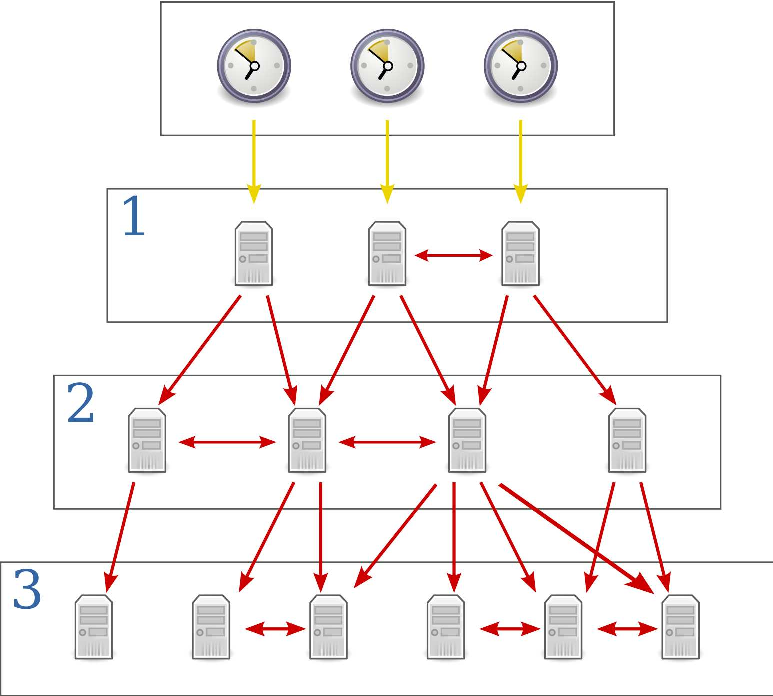
\includegraphics[width=10cm,keepaspectratio]{fig/Network_Time_Protocol_servers_and_clients.pdf}
  \caption{Topology and Hierarchy of NTP}
  \label{fig:ntp-hierarchy}
\end{figure}


\section{Time and timestamps}\label{sec:ntp-time}
NTP always uses the Coordinated Universal Time (UTC).
UTC is maintained by the International Bureau of Weights and Measures in Paris, France.
It is the time scale that forms the basis for the coordinated dissemination of standard frequencies and time signals~\cite{bipm-utc}.
The time specified by UTC is the same for all timezones.
Its calculation is the same as with Greenwich Mean Time (GMT) however
the daylight savings are not accounted. %TODO: CITATION
The UTC scale is adjusted by the insertion of leap seconds to ensure approximate
agreement with the time derived from the rotation of the Earth~\cite{bipm-utc}.
%TODO: better defintion

The leap second is 
These leap seconds are inserted on the advice of the International Earth Rotation and Reference Systems Service (IERS)~\cite{bipm-utc}.
NTP is well designed for leap second occurance.
There is Leap Indicator field
in the structure of NTP packet and there are also fields intended for
information about leap second in structures NTP algorithm uses~\cite{rfc5905}.

The system time is represented by the system clock maintained by
the hardware and operating system.
The goal of the NTP algorithms is to minimize
both the time difference and frequency difference between UTC and the system clock.
When these differences have been reduced below nominal
tolerances, the system clock is said to be synchronised to UTC~\cite{rfc5905}.

The NTP and POSIX timescales are based on the UTC timescale,
but not always coincident with it~\cite{ntp-leap}.
The origin of the NTP timescale, the prime epoch, is 00:00:00 UTC on 1 January 1900,
while the prime epoch of the POSIX timescale is 00:00:00 UTC on 1 January 1970~\cite{ntp-leap}.
Both timescales reckon in seconds since the prime epoch.
For instance, upon the first tick of UTC on 1 January 1972 the NTP clock read 2~272~060~800,
representing the number of seconds since the prime epoch.
% TODO table with ntp time stamps

NTP manipulates with the time through timestamps - a record of UTC time.
NTP timestamp has two fields. The seconds field expressing the number of seconds
and the fraction field expressing fraction of a second~\cite{rfc5905}.
It has never been a goal of NTP to take care of local time,
it is up to operating system to provide user the correct local time~\cite{ntp-overview}.

\section{Network}\label{sec:ntp-network}
Network specification of NTP defines that
the protocol uses the User Datagram Protocol (UDP) on port number 123~\cite{rfc5905, ianna-ports}.
Reliable message delivery such as TCP can actually make the delivered NTP packet less reliable since retries
would increase the delay value and other errors~\cite{rfc5905}.
This is mostly due to overhead of communication with TCP on transport layer.

Because of network latency the timestamp recieved will never be corresponding to
the actual time.
One of the main goals of NTP is to deal with the network latency~\cite{ntp-overview}.

\subsection{Packet structure}\label{subsec:ntp-packet}
As mentioned in~\ref{sec:ntp-time} there are two parts of timestamp.
The 64-bit timestamps used by NTP consist of a 32-bit seconds part and a 32-bit fraction part.

\section{Algorithms}
NTP uses the intersection algorithm for selecting the possible most exact timestamp recieved
from various servers.
